\documentclass[11pt]{article}

\usepackage{underscore,amsmath,amssymb,graphicx}
\usepackage{algorithm}% http://ctan.org/pkg/algorithms
\usepackage{algpseudocode}% http://ctan.org/pkg/algorithmicx


\title{Toward million communicating threads}
\author{Hoang-Vu Dang \and Marc Snir \and William Gropp}

\begin{document}
\maketitle

\abstract{
  We present the design, implementation and analysis of an efficient runtime
  which supports of million concurrently communicating threads using Message
  Passing Interface.
}

\section{Introduction}
Message Passing Interface (MPI) has been implemented by several vendors. On
Blue Gene machine, MPICH is the de-factor implementation, likewise on
Infiniband machine, we have MVAPICH. Cray has their own implementation called
CrayMPI; Intel similarly implements IntelMPI. OpenMPI is an effort of
Open-source commmunity. Each of the implementation uses their best knowledge of
the underlying computing machine and network architecture to optimize their
code. For examples, the implementation might reduce latency by accessing
directly the low-level network-API or optimize critical path using specialized
instructions to reduce cache misses.

Recently, because of the increasing in the number of processor cores within a
computing board, there raises a need of running MPI efficiently in a threaded
environment.  Although MPI specification requires all of its procedures to be
thread-safe, MPI implementations have little concerns for using multiple
threads. For example, OpenMPI latest version still does not provide a stable
support of MPI\_THREAD\_MUTLIPLE.  MPICH suports thread-safety via a
coarse-grain locking which essentially serialized all MPI code. The research to
remove these coarse-grain locks is still undergoning, but the progress is slow
because the existing software stack is only optimized for single-core
performance. For an example, there are significant number of global variables
shared among various component of a MPICH. Global variables which implements
stack, queue or hash-table can be replaced with concurrent data structure,
others might be protected with finer-grains lock. 
However, locks and concurrent data structure has overhead could be added to  
the critical path and reduces performance of single-threaded applications.

Communication in multiple threads could also cause cache trashing or false
sharing if not carefully be taken care of. Moreover, the processor can becomes
under-ultilize because threads execute I/O operations can be preempted. Last but
not least, kernel thread context-switching is costly. Several paper has report
significant overhead for performing MPI concurrently in different thread.

Because of the lack of efficient multi-threaded implementation, to our best
knowledge, there is no production application that uses the thread-safety
feature of MPI. What has been ended up is applications runs MPI in a
single-thread mode, and threads are used only for computation. This leads to a
restrictive programming model similar to Bulk Synchronous Programming (BSP), in
which communication and computation code appears in different phases. This
approach often uses MPI non-blocking feature to allow some overlapping between
phases and hope the MPI runtime will be able to execute communication code
behind the scene. In practice, to support better asynchronous communication
user of MPI implementations often need to enable a flag to request the runtime
to spawn a dedicated polling thread for progressing the communication (e.g.
MPICH_ASYNC_PROGRESS flag in MPICH/MVAPICH).

The solution that we have seen for existing MPI implementation to adopt
multi-core machine is thus ad-hoc and inefficient. In this
paper, we present an approximate implementation of MPI point-to-point
communication which takes into account of multi-core machine by design. Our
implementation is approximate since we shall relax some semantics requirement
of MPI. We argue that our design and algorithms for this relaxation is able to
achieve efficient implementation, yet do not restrict applications from using
MPI effectively. By using this bottom-up strategy, we provide an insight on 
on the cost to support a complete MPI, accurately to the number of memory
accesses.

\section{Runtime Architecture}
\subsection{High-Level System Design}
We first identify the complication of MPI code is on the message matching
mechanism. MPI point-to-point procedures (Send/Recv) facilitate matching
messages by tagging each with an integer in addition to destination and
communicator. The implementation uses several queues data structure to store
incoming requests and messages. For example, the unexpected queue store arrived
messages without a matching request; the posted queue will store the pending
requests without matching messages. Depending on different arrival order,
traversing, insertion or deletion of entries into queues will be issued. In a
concurrent setting, these are critical section that need to be protected. An
efficient lock-free control of these operations are non-existent even though
individual queue could be implemented efficiently.  Moreover, when the number
of concurrent communication increases, traversing a queue requires linear time
to the size of pending requests.

We propose an implementation MPI based on the following assumptions:
\begin{itemize}
  \item Large number of concurrent threads Threads are lightweight; they are
    scheduled by a user-space scheduler that understands synchronization
    objects.
  \item The implementation is optimized for the case where don't cares are not used.
  \item No concurrent send and receive having the same signature, thus we do not yet worry about odering.
  \item The Network Interface Controller (NIC) supports multiple, independent channels.
  \item The NIC can be accessed in user space; it has its own routing tables,
    in order to translate ranks in MPI\_COMM\_WORLD to physical node addresses;
    it has page tables, in order to translate virtual addresses to physical
    addresses.
\end{itemize}

The key data structure for communication is a lock-free hash table which stores
both unsolicited incoming messages and outstanding receives. Since we assume
there are no don't cares, we can hash by source and tag. We focus on critical
operations the creation of communicators or of datatypes is not (yet)
addressed. We also ignore, for the time being, one-sided operations.

The runtime is an integrated system of a user-level thread (ULT) scheduler and
a communication server. The ULT provides a low latency thread management while
the server is a kernel-thread dedicating to message delivery. The two
components interact using the afortmentioned hash-table.  Our primary goal is
to design an algorithm and optimize to minimize the latency of this
interaction. A failure to achieve this goal simply adds extranous overhead to
single threaded application and might not achieve significant benefit that
justifies its cost. We shall also show that our design allows optimization space
to be reduced to optimizing a few neccessary operations.

Resource management is another important issue. Aside from communication
context such as connections and NIC-provided control data which we maintains
per communication server, we have to maintain a pool of packet structure. The
pool is the second shared data structure of the runtime.  Each packet is used
for storing control and message data to deliver to network device.

\begin{figure}
  \centering
  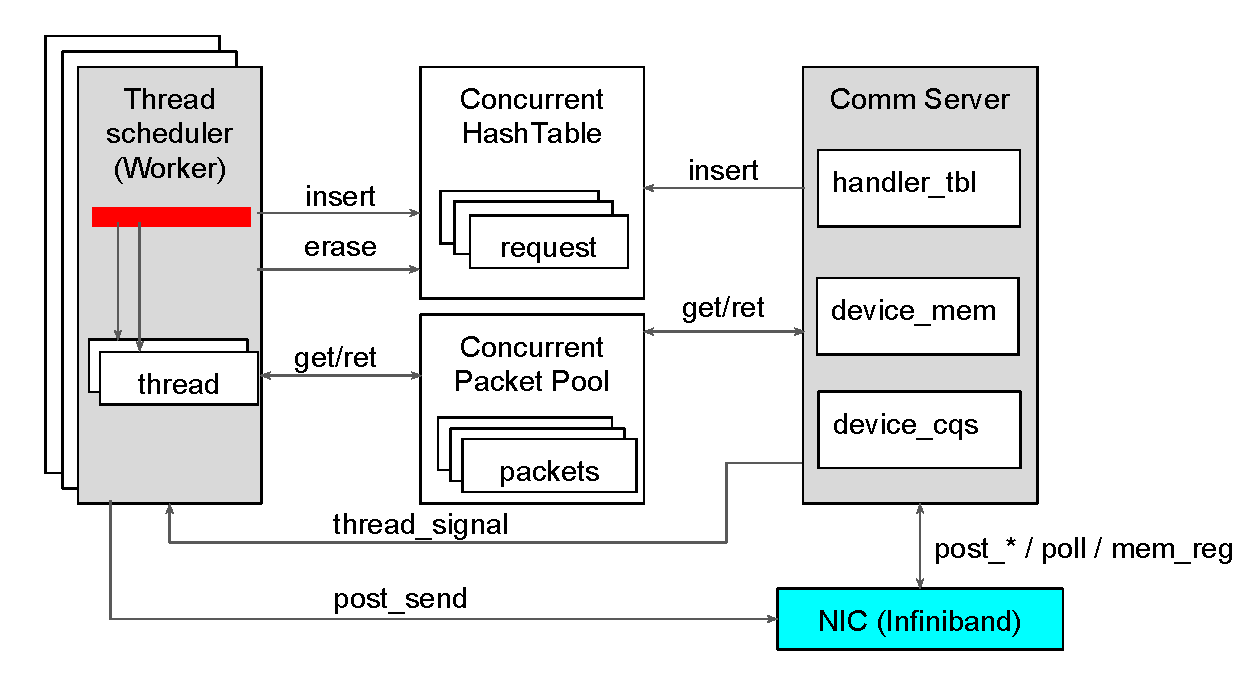
\includegraphics[width=\textwidth]{fig/runtime.pdf}
  \caption{MPI Runtime Architecture for multi-threaded executions}\label{fig:overall}
\end{figure}

Figure \ref{fig:overall} shows the overall architecture of our described
runtime system.

\subsection{Point-to-Point Message Passing Algorithms}
We now describe an algorithm and its data structure that facilites the
point-to-point communication in Message Passing semantics. Our algorithm relies
on a specialized concurrent hash-table $H$ defined as follows.

We denote a tuple $(k,v) \in H$ when $v$ is stored in the hash-table using the
key $k$. At initialization, for any key $k$, only the tuple $(k,\bot)$ are
stored in the table. The hash-table has two operations: 

\begin{itemize}
  \item $H.\text{insert}(k,v)$: attempt to store $(k,v)$ into the hash-table.
  \item $H.\text{empty}(k)$: replace any value stored using key $k$ with $\bot$
\end{itemize}

Additionally, let $H_t$ denote a state of $H$ in real time $t$, $H_{t_0}$ denote the
state of $H$ before a operation and $H_{t_1}$ denotes the state of $H$ after a
operation; $\mathbb{K}, \mathbb{V}$ denote the key and entry space. In a
sequential history, we have the following legal semantics:

\[
  \text{insert}(k, v) = \left\{
    \begin{array}{@{}l@{\thinspace}l}
      v \iff (k,\bot) \in H_{t_0}, (k,v) \in H_{t_1}\\
      v' \iff (k,v') \in H_{t_0}, (k,v') \in H_{t_1}
    \end{array}
    \right.
\]
\[
  \text{empty}(k) = \text{success} \iff  (k,v) \in H_{t_0}, (k,\bot) \in H_{t_1}
\]
\[
  \forall k_0 \in \mathbb{K}, \nexists {v_1, v_2 \in \mathbb{V}}
    \mid {{v_1 \ne v_2} \wedge {(k_0, v_1) \in H_{t} \wedge (k_0, v_2) \in H_{t}}}
\]

That is, the insert is only successful if the entry being stored with $k$ at
the time of insertion is $\bot$.  In that case, $(k,\bot)$ is replaced with
$(k, v)$. Otherwise, the operations fail and existing value is returned i.e. no
changed are made to $H$. In constrat, the erase is always success, which shall
replace any value stored with the input $k$ with $\bot$, essentially removing
the entry from table.  The last point is the consistency requirement, which
means for each key, we can find only one value associated with that key.

In a concurrent setting, we further require the hash-table to be
\textit{linearizable}.  This means we ensure firstly safety and correctness
property. Secondly, we ensure operations takes affect in a real-time order.
This is a strong guarantee however is neccessary to implement MPI semantics
which have operations executed in program order. Lastly, linearizability is 
\textit{composable} which allows us to correctly use the hash-table to implement
other concurrent objects.

Message delivery in general can be implemented in two way: eager or rendevouz
protocol. Eager protocol is when the message buffer is copied into an
intermediate buffer - usually packed with other control data to deliver to the
network. This allows the Send operation to return immediately as the buffer
can be reused.  This protocol however becomes inefficient when message size
gets larger, typically larger than the L2 or L3 cache size i.e. the cost of
data movement is significant.  When this is the case, we switch to rendevouz
protocol in which the data is delivered directly from the source buffer to the
target buffer by the NIC thus saving extra copies.  The protocol however requires
some control messages to exchange control data and signal completion.

\subsubsection{Point-to-Point Eager protocol}

\begin{algorithm}
  \caption{Eager-message send/recv for thread}
  \label{algo:short}
  \begin{algorithmic}[1] % The number tells where the line numbering should start
    \Procedure{Send-Eager}{$b, s, d$} \Comment: buffer, size, destination signature 
      \State $p$ = pkpool.get()
      \State Set packet header $p.d$ to $d$
      \State Copy $b$ to $p.b$
      \State Post $p$ to network for send.
    \EndProcedure
    \\
    \Procedure{Recv-Eager}{$b, s, d$} \Comment: buffer, size, source signature 
      \State $\Gamma$ = current thread id.
      \State Create a request $r$ = $(b,s,d,\Gamma)$
      \State Create hash-value $v$ from $r$.
      \State Create hash-key $k$ from $d$.
      \State $v' = H.\text{insert}(k,v)$
      \If {$v' \ne v$}
        \Comment: insertion fail, message has arrived, copy the data.
        \State Copy $v'.p.b$ to $b$
        \State pkpool.ret($p$)
      \Else
        \Comment: insertion success, message has not arrived.
        \State \texttt{ThreadWait}()
      \EndIf
      \State $H.\text{erase}(k)$
    \EndProcedure
  \end{algorithmic}
\end{algorithm}

\begin{algorithm}
  \caption{Eager-message packet handler for communication server}
  \label{algo:server-short}
  \begin{algorithmic}[1]
    \Procedure{Recv-Eager-Packet}{p}
      \State Create hash-value $v$ from $p$.
      \State Create hash-key $k$ from $p.d$.
      \State $v' = H.\text{insert}(k,v)$
      \If {$v' \ne v$}
        \Comment: insertion fail, thread has arrived, copy the data.
        \State Copy $p.b$ to $v'.r.b$
        \State \texttt{ThreadSignal}($r.\Gamma$)
        \State pkpool.ret($p$)
      \Else
        \Comment: insertion success, thread has not arrived, nothing to do.
        \State \Return
      \EndIf
    \EndProcedure
  \end{algorithmic}
\end{algorithm}

The algorithm for eager protocol is listed in Algorithm \ref{algo:short} and
\ref{algo:server-short} for worker thread side and communication server side
respectively. The basic idea here is that the thread and the communication
server at the receiving side can effectively coordinating to match messages and
requests.

If the communication server succeeds with the hash insertion, the receiving
request has not been posted by a thread, the server return immediately. A
thread later comes, eventually fail the insertion but find a packet
with the needed data to copy to its buffer.

On the other hand, the thread is the one who succeeds and the request is
inserted into the hash-table with the synchronization object. The thread yield
by executing \texttt{ThreadWait}. When the eager packet arrived, the
request handler is executed by the communication server. The server will fail
the insert but find the request with the attached synchronization object. It
now can wake up the thread using \texttt{ThreadSignal}. In this situation,
there is a locality consideration whether the thread or the server should
perform the memory copy. However, this is an optimization which does not effect
the correctness of our algorithm.

\subsubsection{Point-to-Point Rendevouz protocol}
A rendevouz protocol have the same algorithm as short protocol after we have
exchanged the control message via eager-protocol. The control messages 
includes two messages: a RTS (ready-to-send) issued by the sender, a RTR
(ready-to-receive) issued by the receiver. By then, the sender and the receiver
has known the addresses of each other buffer and they can perform
communication.  The data transfer could be optimized further using the
Remote Direct Memory Access (RDMA) feature of modern Network Interface
Controller (NIC).  Several researchs has focused on optimizing this operation.

In our runtime, we can save one control message i.e. the RTS.  The reason is
we do not have wird-card, the sender and receiver knows exactly their target.
We only require the receiver to send its buffer to the sender. The sender can
follow up by issuing an RDMA.  Analogous to the eager protocol, whenever the
sender or receiver is required to wait for a matching message it will perform
\texttt{ThreadWait}, and later when the message has arrived the communication server
will perform a \texttt{ThreadSignal}.

Specifically, the sender waits when the RTR message has not arrived or when
RDMA is pending. In both situation the server wake up the sender thread when
RDMA has completed. The receiver after issuing the RTR will wait until the
signal that RDMA has finished arrived and data is now available.

\subsection{Critical Operations Discussion}
Clearly, optimizing the hash-table, packet pool and thread operations is the
key to the performance of both protocol. One could achieve $O(1)$ amortized
complexity.  However, an efficient implementation requires optimizing for the
constant factor. Ideally, we want these operation to be \textit{wait-free} to
ensure progress and the constant factor is tiny. In the next section, we
describe the implementaion of each of the component and show how we could
optimize to reduce the cache misses in NUMA achitecture.

\section{Implementation and Optimization}
\subsection{Thread scheduler}
Our thread scheduler is implemented as a User-Level Thread (ULT) in order to
minimize context switching overhead. The context-switching mechanism is similar
to that of Argobots and Boost coroutines, we make use of \texttt{fcontext}. The
idea is to maintains a separate stack for each thread. A few registers
(including the program counter) is saved and restored from an allocated space
in the stack. Morever, the switch is designed to not involve OS system call,
thus by-passing the kernel. This overall reduces the latency of switching to a
new context to under a hundred cycle.

Rather than designing a general purpose ULT, we focus on the two most important
operations: \texttt{ThreadWait} and \texttt{ThreadSignal}. One possible
implementation is condition variable. This is the typical synchronization often
used in POSIX thread, and other ULT library such as Argobots.  However, these
are expensive since condition variable in general requires a lock. A
busy-waiting implementation is even worst since the processor spends useless
time polling. Qthreads uses a slight modification notion i.e.  full-empty bit.
However, internally each full-empty bit object is a waiting queue and
rescheduling requires traversing this queue to place them back to the run
queue.

Our thread scheduler achieves wait-freedom for both afortmentioned operation.
Except the required context-swiching for \texttt{ThreadWait}, each operation is
simply a single x86 instruction. The idea behind our thread scheduler is a novel
use of bit-vector. Rather than using a queue to implement a set of runnable thread,
each bit in the bit-vector indicates a thread is runnable.

When a worker is created, it is given a unique worker id, denotes as $\omega$.
When a thread is created by a worker, it is assigned an unique id $\Gamma$
within the range of $[0,M-1]$, for $M$ is the maximum concurrent threads for
that worker.  For example, using a vector of $8$ 64-bit words, we allow up to
$512$ concurrent threads per worker.

A pair $(\omega, \Gamma)$ uniquely defines a thread in the system at a point in
time. Additionally, during the creation time, the worker atomically set the
associated $\Gamma$ bit.

\begin{algorithm}
  \caption{Thread scheduler}
  \label{algo:thread}
  \begin{algorithmic}[1]
    \Procedure{Scheduling}{w, V} \Comment{worker, bit-vector}
    \While {!w.stop} \Comment{loop until user ask to stop}
      \For{word64 in V}
      \If{word64 $\ne$ 0}
        \State localWord64 = 0
        \State ATOMIC_EXCHANGE(word64, localWord64)
        \While {localWord64 $> 0$}
          \State b = Find-First-Set(localWord64)
          \State FlipBit(localWord64, b)
          \State ContextSwitch($\Gamma_{b}$)
        \EndWhile
      \EndIf
      \EndFor
    \EndWhile
    \EndProcedure
  \end{algorithmic}
\end{algorithm}

\begin{algorithm}
  \caption{Thread Operations}
  \label{algo:thread-ops}
  \begin{algorithmic}[1]
    \Procedure{ThreadWait}{sync}  \Comment{Synchronization object}
      \State sync = {$(\omega, \Gamma)$}
      \State ContextSwitch($\omega$)
    \EndProcedure
    \\ 
    \Procedure{ThreadSignal}{sync} \Comment{Synchronization object}
      \State w = sync.$\omega$
      \State ATOMIC_SET_BIT(w.V, sync.$\Gamma$)
    \EndProcedure
  \end{algorithmic}
\end{algorithm}

Algorithms \ref{algo:thread} describes our scheduling algorithms. The
scheduler, when being free will look at each 64-bit word in the bit-vector to
find a schedulable thread.  Instead of working at 1-thread granularity, we work
at 64-threads represented by a 64-bit word. By using an atomic exchange to swap
the interested word to local variable, we are able to continously perform read
and write this variable without accessing the main memory.  This is not only
easier for correctness since concurrent threads are writing to the same
bit-vector; this also ensures progress property for all threads because we
can schedule them in order. We do not support thread-stealing yet, but it can
be done by allowing stealing 64-bit word.

Algorithms \ref{algo:thread-ops} describes the two thread operations.
\texttt{ThreadWait} simply stores the thread indentification i.e. ($(\omega,
\Gamma)$) into the synchronization object and switch back to the worker
scheduler. On the other hand, \texttt{ThreadSignal} shall access the
bit-vector and atomically set the bit in the appropriate word based on the
the same information stored in the synchronization object.

Note that \texttt{ThreadWait} is executed in the same kernel thread as the
thread scheduler associating with the running ULT, thus there is no race that
we need to worry about in accessing the bit-vector. \texttt{ThreadSignal} can
be executed anywhere, and in our design it will be executed by the
communication server. Thus in the algorithm it is errornous to perform
\texttt{ThreadSignal} multiple times on the same object. In practise, we store
additionally an atomic flag per synchronization object to prevent this to
happen.

There are two possible problems with the described thread scheduler design.
Firstly, the performance degrades greatly when we support a large number of
threads. The reason is we have to iterate over the bit-vector. Secondly, there
could be an issue with fairness because thread with larger bit-index will be
scheduled later.

We currently ignore the fairness issue, and as long as we maintain the progress
property this is not a big problem. We tackle the first problem by using a
hierachical design of bit-vector.  That is, we could use a secondary bit-vector
as a hint to index into the first level bit-vector.  Specifically, each bit in
the secondary bit-vector indicates which word in the first level could have
schedulable thread. More specifically, \texttt{ThreadSignal} will perform a bit
set first into the first level then a bit set into the second level. The
scheduler will first look into the second level to find a potentially word and
go directly to that word index to look for schedulable threads. It can happen
that the secondary might indicate the thread is schedulable, but when it comes
to the first level the thread is already scheduled by the previous check.  This
\textit{false positive} happen because the secondary level bit is potentially
shared a group of thread. However, it does not affect the correctness since the
thread will not be scheduled twice in any situation.

Using this scheme, if we use 1 word for the secondary level bit-vector, each
bit represent a 64-bit words in the first level, each worker can support up to
$4096$ threads. And since eight words can fit in a cache line and better to read
together, we can use 1 bit to represent a set of eight 64-bit words. Similarly by having
eight words in the secondary level we can support $262144$ concurrent threads per
worker. Therefore, with a small number of worker, we can go up to our goal of
million thread without sacrifying much performance.

\subsection{Concurrent Hash-Table}
Our concurrent hash-table is not deviated very much from conventional
concurrent hash-table. We however find opportunity to optimize further by taking 
advantage of some semantics requirement that we have mentioned.

Firstly, we use a spinlock per bucket. This is an viable option since we could
control the table size to reduce the hash collision to minimal. The table size is
related directly to how many concurrent operations which is controlled by 
our packet pool size. Since the collision is minimal, the conflict can only happen
between communication server and a thread when both try to insert into the same
bucket at the same time. Since there is only synchronization between 2 threads
a spinlock is sufficient for our purpose moreover allowing a very simple design.

Secondly, we design each bucket as an 4-entry array. Each entry consists of 2
64-bit words. Within a 4-entry array, one will be used as control entry and the
other three are used for storing a pair of key and data. The control entry has
an atomic flag for spin locking, and a pointer to point to the next bucket in
case we have more than 3 collisions. Since a bucket typically fits in a cache
line, we suffer only 1 cache miss at most when trying to lock the bucket and
the data can be read without more cache misses.

Lastly, the \texttt{insert} operation returns the address of the associated
entry. This allows the \texttt{empty} operation to be a single instruction,
which set the key to $\bot$. This is only possible because only one thread can
change an entry key because no concurrent Send/Recv with the same tag is allowed.

Therefore our \texttt{empty} is lockless and achieves wait-freedom too. Our
\texttt{insert} is cache-friendly and typically also wait-freedom with high probability 
when the table size is large enough (thus with little to no hash collision).

\subsection{Concurrent Packet Pool}
Our pool is currently implemented using a lockfree stack. At the
initialization, a fixed numbers of packet is allocated and push to the stack.
During runtime a pool \texttt{get} is a stack \texttt{pop} and a pool
\texttt{ret} is a stack \texttt{push}.

Since the packet is a unit of communication, its data is read and written very
frequently. The stack implementation although does not give us the best latency
in terms of concurrent accesses, it gives us good temporal locality of the
packet data.

The pool is also served as a mechanism to control the concurrency level of the system.
A thread will yield control when there is no available packet.

\section{Experiment}
\subsection{Thread Scheduler}
\begin{figure}[h]
  \centering 
  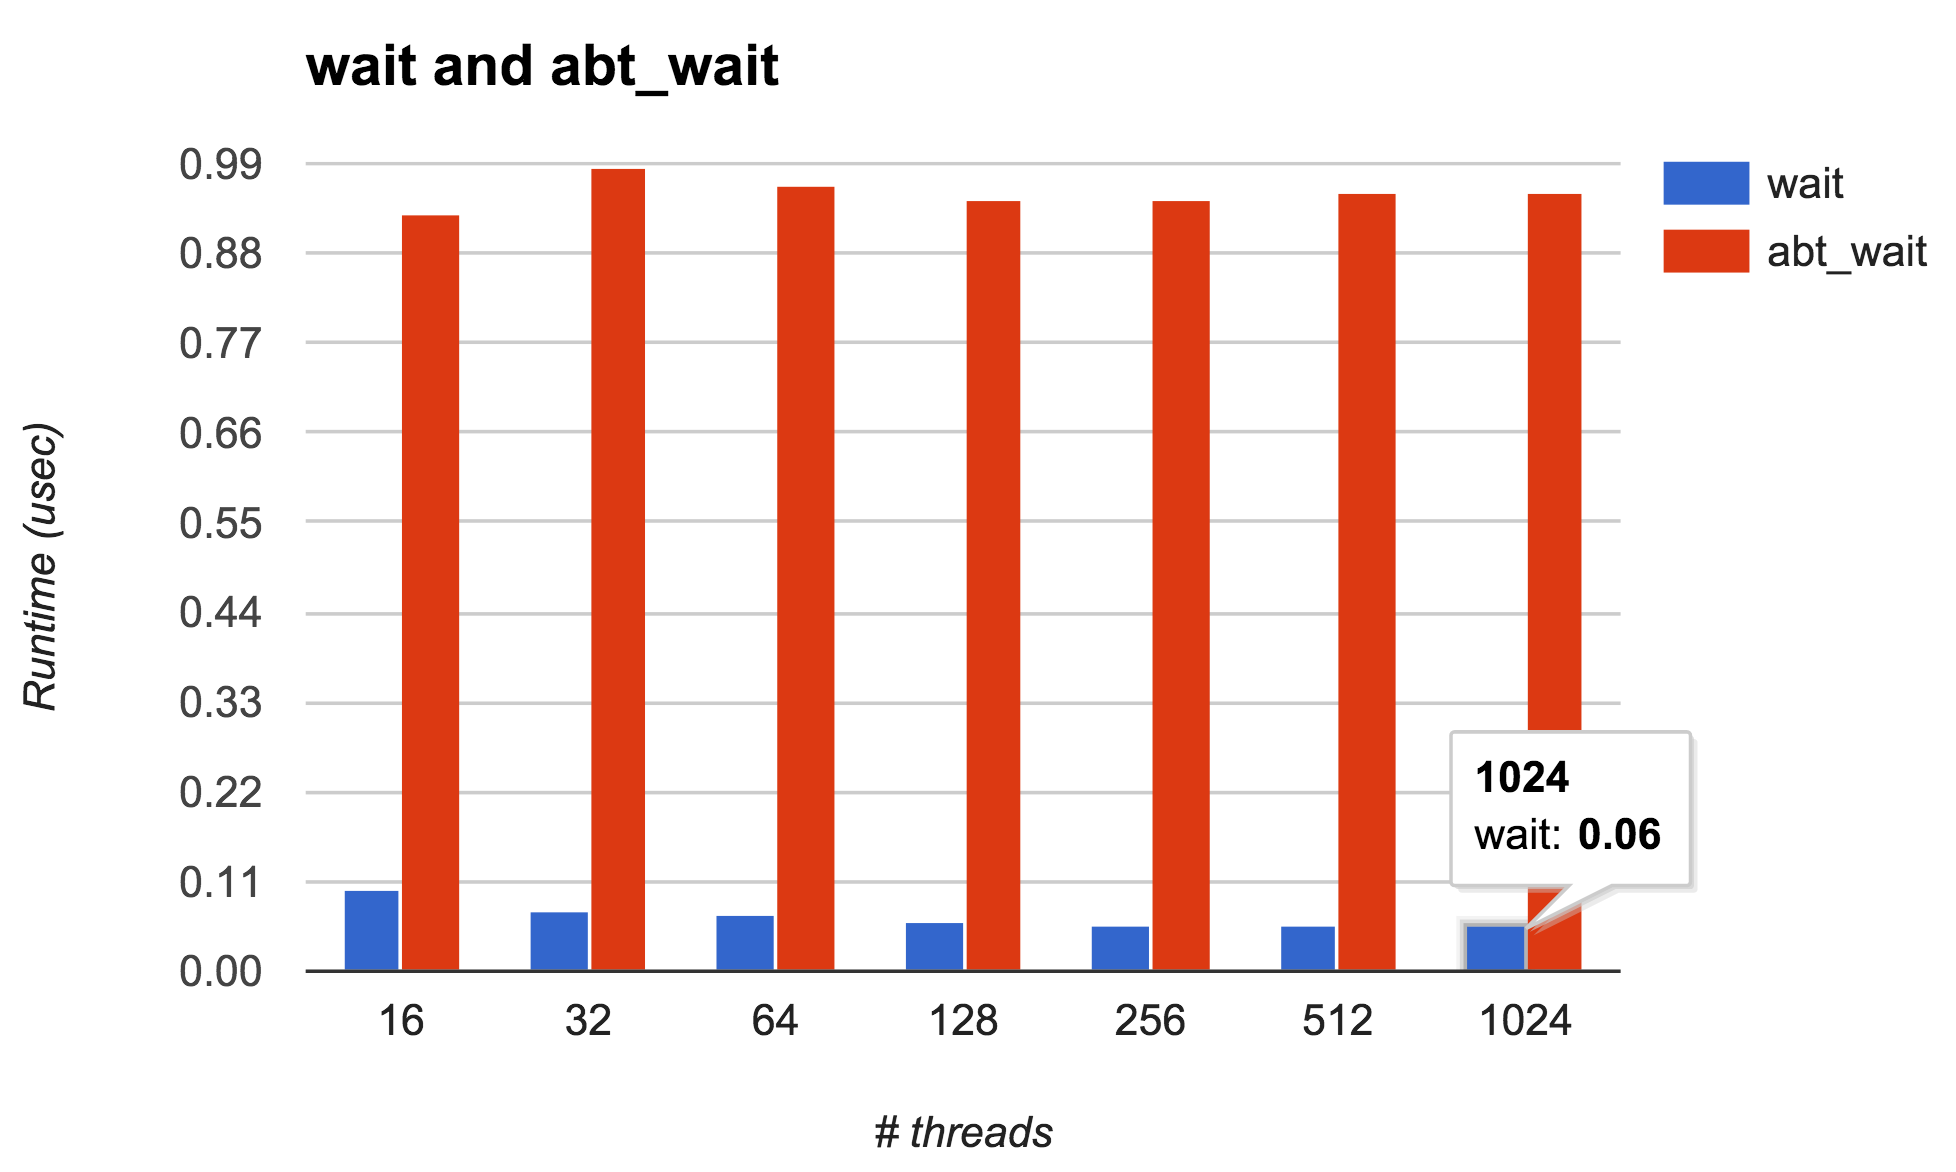
\includegraphics[width=0.9\textwidth]{fig/thread.png}
  \caption{Comparing Thread wait and signal with Argobots condition variable
  implementation. Runtime from entering wait until waken up by signal per thread.}

\end{figure}

\newpage

\subsection{Concurrent Hash-Table}
\begin{figure}[h!]
  \centering 
  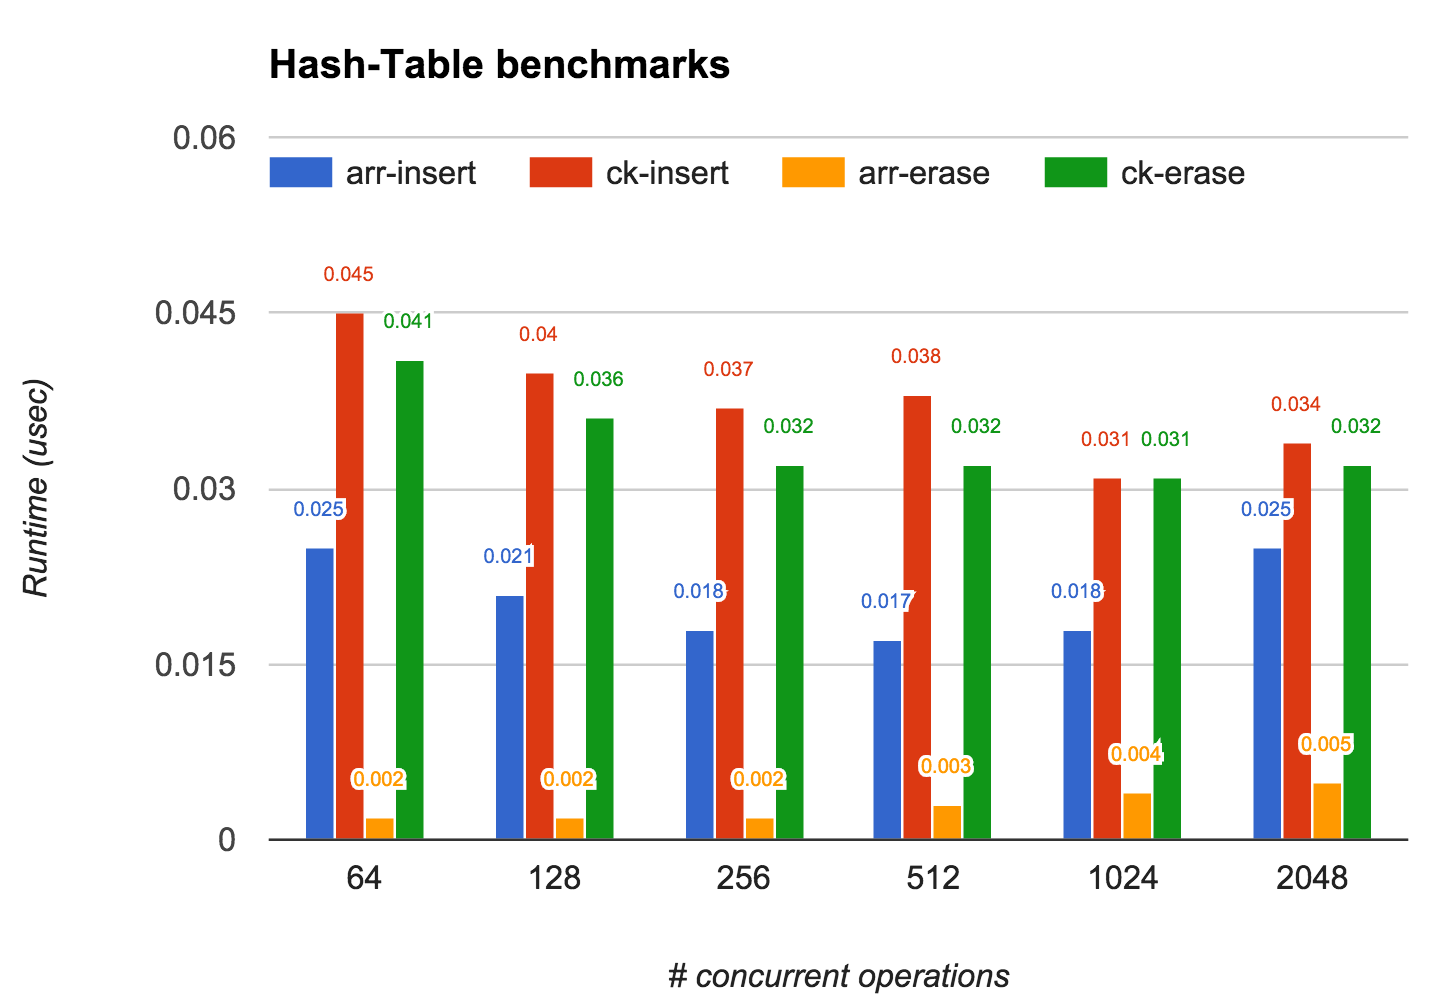
\includegraphics[width=\textwidth]{fig/hashtbl.png}
  \caption{Comparing hash-table inserting and deletion by concurrent threads
    with cuckoo-hasing.  Runtime is averaged per operation per thread.
    \texttt{arr} suffix is our implementation and \texttt{ck} prefix is cuckoo-hasing}.
\end{figure}

\newpage

\subsection{Overall overhead}
\begin{figure}[h!]
  \centering 
  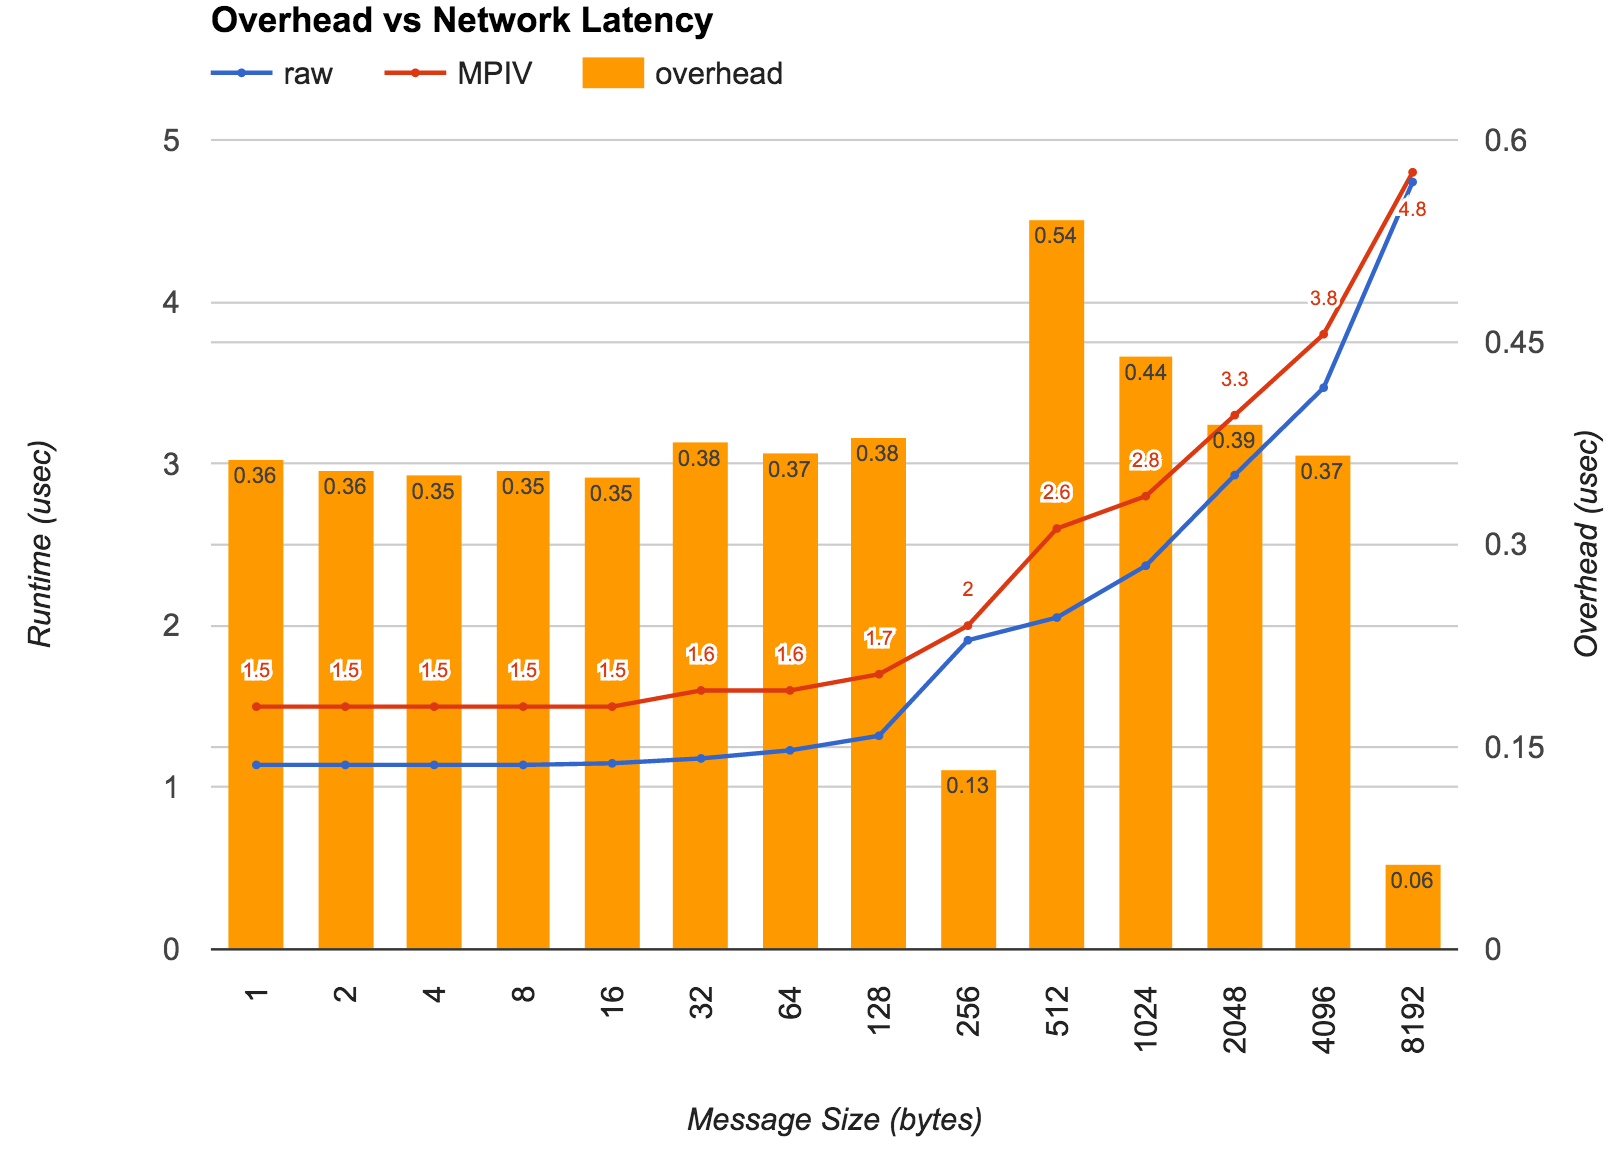
\includegraphics[width=\textwidth]{fig/overhead.png}
  \caption{Total overhead of runtime system, comparing to raw network latency.}
\end{figure}

\subsection{Pingpong multiple threads}
\begin{figure}[h!]
  \centering 
  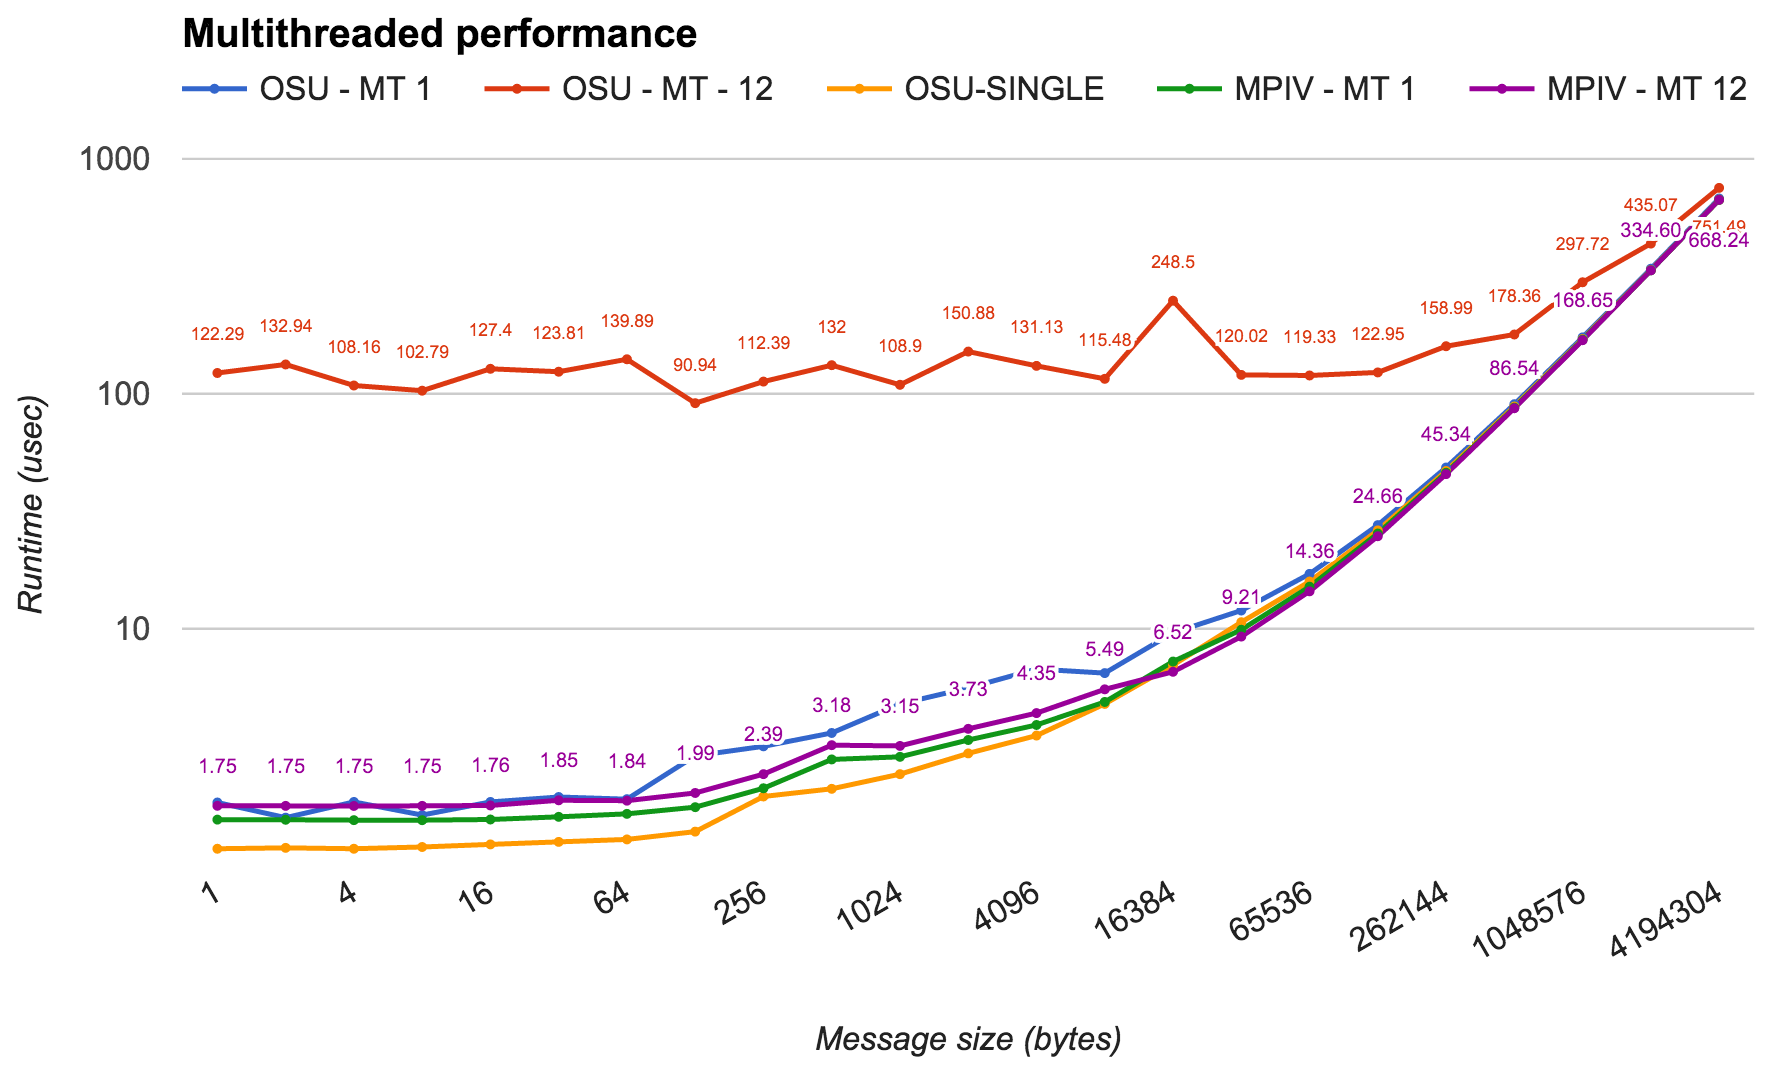
\includegraphics[width=\textwidth]{fig/pingpong.png}
  \caption{Comparing multi-threaded pingpong with OSU benchmarks using 1-thread
  in 1-worker and 12-threads in 12-workers. MPIV is our implementation.}
\end{figure}

\newpage

\subsection{Applications}
\section{Related Works}
\section{Conclusion}
\end{document}
